\documentclass[aspectratio=169,handout]{beamer}
\usepackage{will_handley_beamer}
\usepackage{title_page}

% Commands
% --------
% - \arxiv{arxiv number}
% - \arxiv{<number>}            arxiv.org/abs/<number>
% - \oldarxiv{<arxiv number>}   arxiv.org/<number>
% - \doi{<doi>}                 doi.org/<doi>
% - \xkcd{<number>}             xkcd.com/<number>
% - \email{<email>}             <<email>>
% - \tthref{<website>}          <website>
% - \av[dist]{<quantity>}       <quantity>_{dist}
% - \student{<name>}{<detail>}{<photo>}

% Talk details
% ------------
\title{Sampling methods for high energy physics \& particle astrophysics}
%\subtitle{<+subtitle+>}
\date{19\textsuperscript{th} August 2024}

\begin{document}

\begin{frame}
    \titlepage
\end{frame}

\begin{frame}
    \frametitle{<+Frame title+>}
    <+Content+>
\end{frame}

\begin{frame}
    \frametitle{The nature of sampling}
    <++>
\end{frame}


\begin{frame}
    \begin{columns}
        \column{0.48\textwidth}
        \begin{block}{\textbf{MCMC}}
            \only<16>{
                \begin{itemize}
                    \item Single ``walker''
                    \item Explores posterior
                    \item Fast, if proposal matrix is tuned
                    \item Parameter estimation, suspiciousness calculation
                    \item Channel capacity optimised for generating posterior samples
                \end{itemize}
            }
        \end{block}
            \includegraphics<1|handout:0>[width=\textwidth,page=16]{figures/himmelblau.pdf}%
            \includegraphics<2|handout:0>[width=\textwidth,page=17]{figures/himmelblau.pdf}%
            \includegraphics<3|handout:0>[width=\textwidth,page=18]{figures/himmelblau.pdf}%
            \includegraphics<4|handout:0>[width=\textwidth,page=19]{figures/himmelblau.pdf}%
            \includegraphics<5|handout:0>[width=\textwidth,page=20]{figures/himmelblau.pdf}%
            \includegraphics<6-15|handout:0>[width=\textwidth,page=21]{figures/himmelblau.pdf}%
        \centerline{\includegraphics<16>[width=0.5\textwidth,page=19]{figures/himmelblau.pdf}}
        \column{0.48\textwidth}
        \begin{block}<7->{\textbf{Nested sampling}}
            \only<16>{
                \begin{itemize}
                    \item Ensemble of ``live points''
                    \item Scans from prior to peak of likelihood
                    \item Slower, no tuning required
                    \item Parameter estimation, model comparison, tension quantification
                    \item Channel capacity optimised for computing partition function
                \end{itemize}
            }
        \end{block}
            \includegraphics<7|handout:0>[width=\textwidth,page=1]{figures/himmelblau.pdf}%
            \includegraphics<8|handout:0>[width=\textwidth,page=2]{figures/himmelblau.pdf}%
            \includegraphics<9|handout:0>[width=\textwidth,page=3]{figures/himmelblau.pdf}%
            \includegraphics<10|handout:0>[width=\textwidth,page=4]{figures/himmelblau.pdf}%
            \includegraphics<11|handout:0>[width=\textwidth,page=5]{figures/himmelblau.pdf}%
            \includegraphics<12|handout:0>[width=\textwidth,page=6]{figures/himmelblau.pdf}%
            \includegraphics<13|handout:0>[width=\textwidth,page=7]{figures/himmelblau.pdf}%
            \includegraphics<14|handout:0>[width=\textwidth,page=8]{figures/himmelblau.pdf}%
            \includegraphics<15|handout:0>[width=\textwidth,page=15]{figures/himmelblau.pdf}%
        \centerline{\includegraphics<16>[width=0.5\textwidth,page=4]{figures/himmelblau.pdf}} 
    \end{columns}
\end{frame}

\begin{frame}
    \frametitle{Nested Sampling}
    <++>
\end{frame}
\begin{frame}
    \frametitle{Lattice QCD with nested sampling}
    <++>
\end{frame}
\begin{frame}
    \frametitle{$p$-values with nested sampling}
    <++>
\end{frame}
\begin{frame}
    \frametitle{Fine-tuning with nested sampling}
    <++>
\end{frame}
\begin{frame}
    \frametitle{Model comparison as quantifying fine tuning}
    <++>
\end{frame}

\begin{frame}
    \frametitle{Conclusions}
    \framesubtitle{\tthref{github.com/handley-lab}}
    \tikz[overlay,remember picture]
        \node[anchor=north east] (A) at ($(current page.north east)+(0,0)$) {
        
\includegraphics[width=0.09\textheight]{figures/students/adam_ormondroyd.jpg}%
        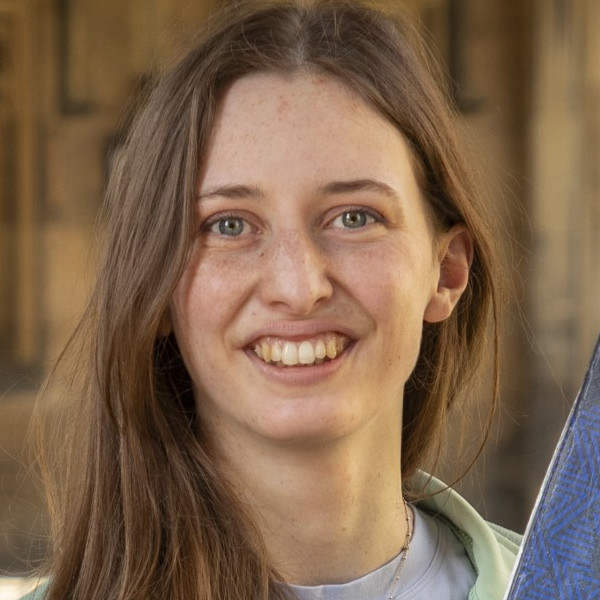
\includegraphics[width=0.09\textheight]{figures/students/charlotte_priestley.jpg}%
        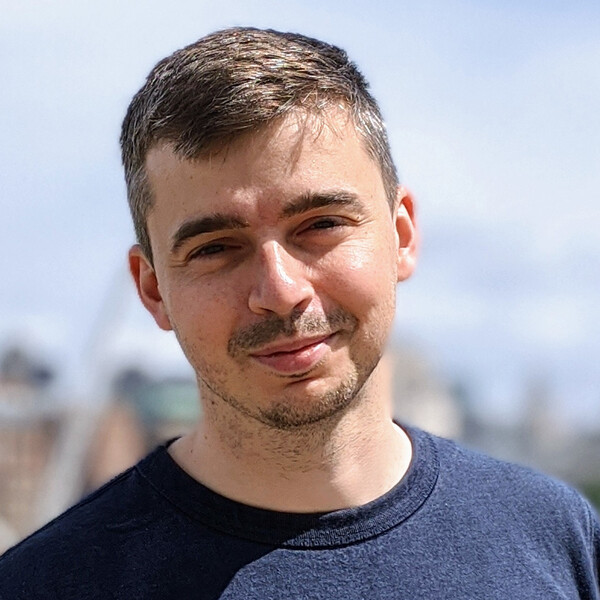
\includegraphics[width=0.09\textheight]{figures/students/david_yallup.jpg}%
        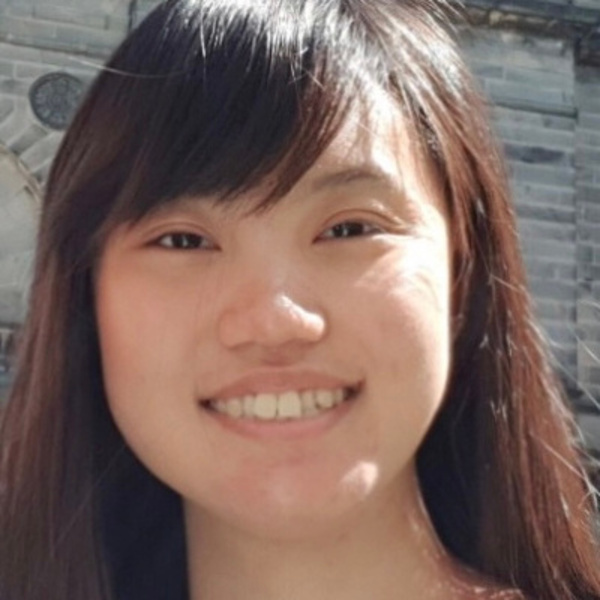
\includegraphics[width=0.09\textheight]{figures/students/dily_ong.jpg}%
        
\includegraphics[width=0.09\textheight]{figures/students/george_carter.jpg}%
        
\includegraphics[width=0.09\textheight]{figures/students/harry_bevins.jpg}%
        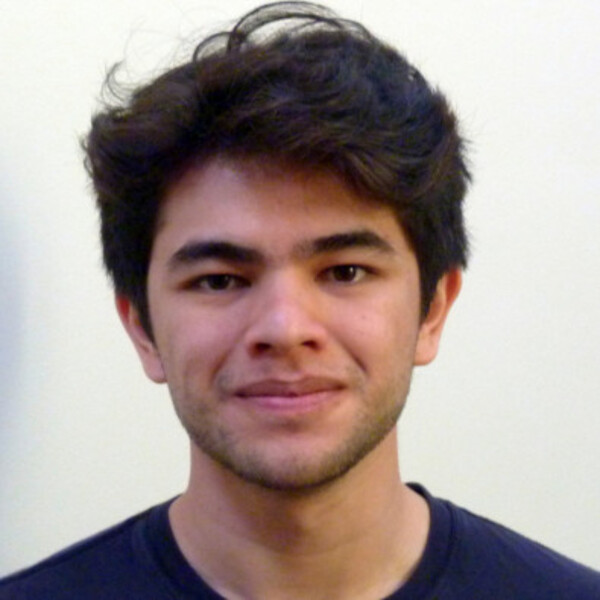
\includegraphics[width=0.09\textheight]{figures/students/ian_roque.jpg}%
        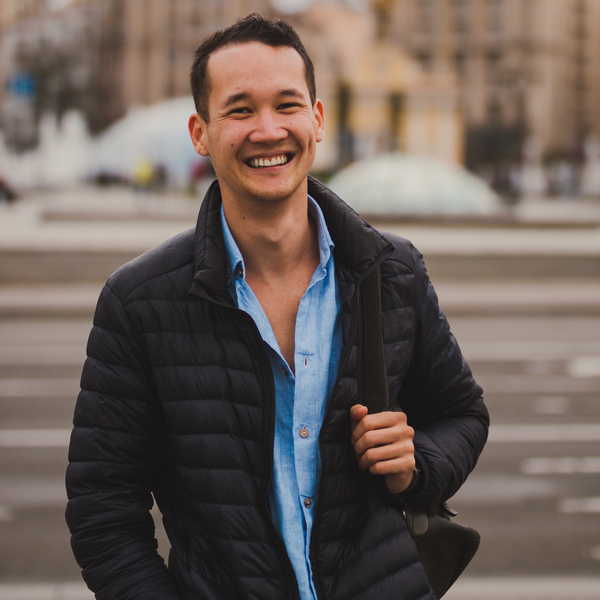
\includegraphics[width=0.09\textheight]{figures/students/kilian_scheutwinkel.jpg}%
        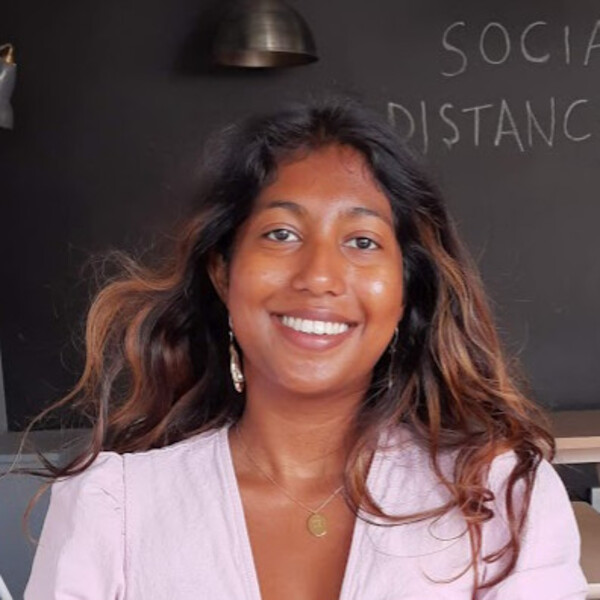
\includegraphics[width=0.09\textheight]{figures/students/metha_prathaban.jpg}%
        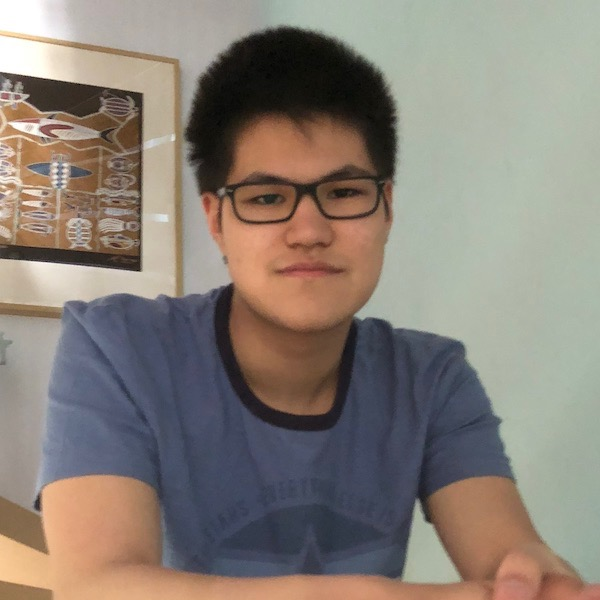
\includegraphics[width=0.09\textheight]{figures/students/namu_kroupa.jpg}%
        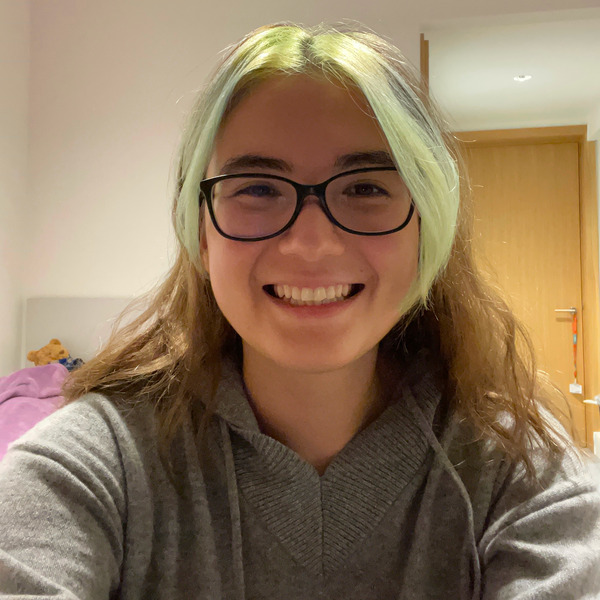
\includegraphics[width=0.09\textheight]{figures/students/sinah_legner.jpg}%
        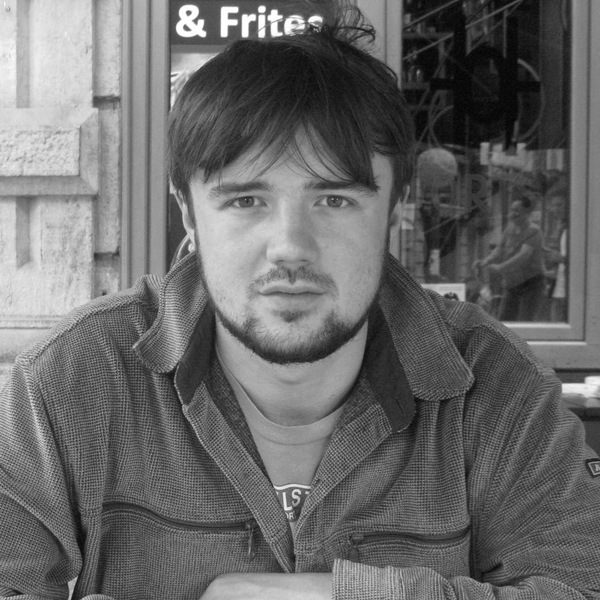
\includegraphics[width=0.09\textheight]{figures/students/sam_leeney.jpg}%
        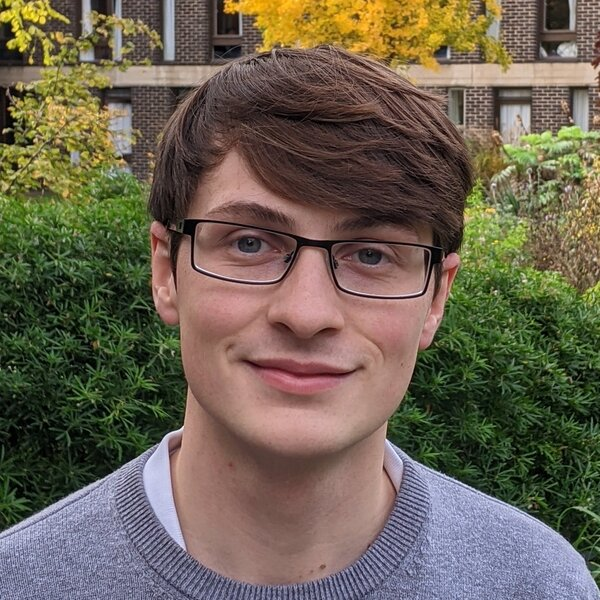
\includegraphics[width=0.09\textheight]{figures/students/thomas_gessey-jones.jpg}%
        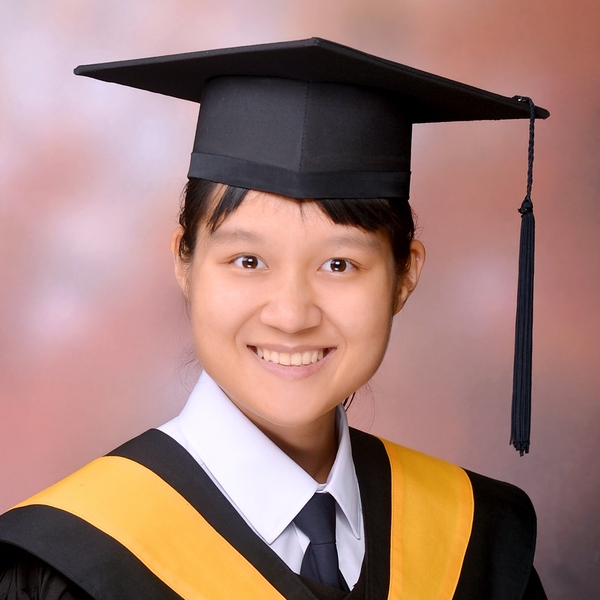
\includegraphics[width=0.09\textheight]{figures/students/wei-ning_deng.jpg}%
    };
\end{frame}

\end{document}
